\documentclass[conference]{IEEEtran}
\usepackage{amsmath,amsfonts,amssymb}
\usepackage{graphicx}
\usepackage{cite}
\usepackage{url}
\usepackage{booktabs}
\usepackage{array}
\usepackage{xcolor}
\usepackage{tikz}
\usetikzlibrary{arrows.meta,positioning,calc,fit}
\usepackage{pgf-umlsd}

\hyphenation{op-tical net-works semi-conduc-tor IEEE-Xplore}

\begin{document}

\title{Toward Reputation Without Revelation: Private and Verifiable Trust In a Decentralized World}

\author{
\IEEEauthorblockN{Antonio M. de Sousa}
\IEEEauthorblockA{\textit{Graduate Program in Computer Science (PGCOMP)}\\
\textit{Federal University of Bahia (UFBA)}\\
Salvador, Brazil\\
antonio.mateus@ufba.br}
\and
\IEEEauthorblockN{Allan E. S. Freitas}
\IEEEauthorblockA{\textit{Graduate Program in Systems and Products Engineering (PPGESP)}\\
\textit{Federal Institute of Bahia (IFBA)}\\
Salvador, Brazil\\
allan@ifba.edu.br}
\and
\IEEEauthorblockN{Leobino N. Sampaio}
\IEEEauthorblockA{\textit{Graduate Program in Computer Science (PGCOMP)}\\
\textit{Federal University of Bahia (UFBA)}\\
Salvador, Brazil\\
leobino@ufba.br}
}

\maketitle

\begin{abstract}
Authentication verifies who an entity is, but not whether it keeps behaving reliably over time. Reputation fills this gap, yet centralized reputation providers are single points of failure, and decentralized ones often expose the very histories they score. We propose a technology-agnostic framework for decentralized reputation, organized into six separate concerns, that reconciles verifiability with privacy and supports two instances: Verifiable Anonymous Reputation and Blind Reputation. We implement the first as ShadowRep, which combines Decentralized Identifiers (DIDs), Fully Homomorphic Encryption (FHE), and Zero-Knowledge Proofs (ZKPs) in a challenge-based protocol with an asymmetric reward and penalty rule, in which proofs are bound on-chain to each round and to each verifier. In a 20-node Edge/IoT emulation over 460 rounds with injected omission failures and on-off attackers, honest proposers obtained a full quorum in 99.5\% of their rounds, nodes with omission failures fell below 10\%, and each attacker defection halved its score and required about 15 honest services before the next one. FHE evaluation costs about 19~ms and Groth16 proof generation about 236~ms per response, roughly 33$\times$ a SHA-256 and ECDSA baseline, plus about 273k gas per on-chain verification, a cost compatible with asynchronous reputation updates.
\end{abstract}

\begin{IEEEkeywords}
Decentralized Reputation, Privacy, Blockchain, Zero-Knowledge Proofs
\end{IEEEkeywords}

\section{Introduction}
Authentication and authorization ensure identity and access control, but they do not guarantee the quality, reliability, or consistency of the services provided over time. Reputation summarizes aspects such as availability, response time, integrity of delivered data, and compliance with Service Level Agreements \cite{fernandes2023blockchain, liu2022vrepchain, 10335003}, and helps identify entities that, although authenticated, act opportunistically, negligently, or maliciously \cite{ZHOU2021155, arshad2022reputable, solomon2023smartfhe}.

Because reputation guides decisions, it is also a target. Concentrating it in identity silos such as Meta, Microsoft, and Google creates single points of failure whose compromise can expose sensitive information or make an agent's reputation unavailable \cite{10891701, ernstberger2023sok, ZHOU2021155, lu2023towards}. Decentralized reputation systems remove this dependency \cite{arshad2022reputable}, but privacy remains a challenge, as agents with high reputation become targets for impersonation, opportunistic exploitation, or reputation poisoning.

Regulation adds a further constraint. Under the GDPR \cite{gdpr2016}, a reputation score linked to an identifiable individual is personal data, deriving it from behavioral history is profiling (Art.~4(4)), and pseudonymized data remains in scope (Recital~26). The regulation also mandates data minimization (Art.~5(1)(c)), data protection by design (Art.~25), and the right to erasure (Art.~17), and Brazil's LGPD \cite{lgpd2018} follows analogous principles. These obligations conflict with designs that record reputation histories in plaintext on an immutable and replicated ledger \cite{finck2019blockchain}, and they also reach IoT devices, which are usually bound to identifiable operators. Computing reputation over encrypted data, anchoring only commitments on-chain, and disclosing predicates (e.g., ``score above a threshold'') instead of raw values is therefore better aligned with these requirements \cite{aronoff2025sok, R2026377}.

We build on decentralized identity, in which DIDs and Verifiable Credentials (VCs) let individuals control and selectively prove claims about themselves \cite{w3c-did, allen2018, 10664246, tan2023survey}, and on ZKPs, so that agents can prove their trustworthiness without disclosing absolute reputation values \cite{surveyprivacypreserving}. Our contributions are:
\begin{itemize}
\item \textbf{A technology-agnostic framework for decentralized reputation based on separation of concerns}, with six layers and two instances: \textit{Verifiable Anonymous Reputation}, in which agents compute their own score over encrypted data and prove predicates about it, and \textit{Blind Reputation}, in which the score is computed collectively via MPC and FHE so that not even its subject knows it.
\item \textbf{A challenge-based reputation mechanism (PoE-FHE)} that realizes the anonymous instance, in which agents prove in zero knowledge that they hold the result of a homomorphic computation, combined with an asymmetric reward and penalty rule.
\item \textbf{ShadowRep, an open-source proof of concept}, evaluated in an emulated Edge/IoT environment from behavioral and computational perspectives, including a comparison against a SHA-256 and ECDSA baseline.
\end{itemize}

\section{Related Work}\label{sec:trabs}
Decentralized reputation has been explored in several domains. Zhou et al.~\cite{ZHOU2021155} propose a blockchain-based reputation system for e-commerce that removes single points of failure, Reputable~\cite{arshad2022reputable} maintains trust collaboratively across blockchain ecosystems, and \cite{10335003} proposes a pseudonymous decentralized reputation system. In vehicular networks, \cite{fernandes2023blockchain} and Vrepchain~\cite{liu2022vrepchain} support reliable data sharing, and \cite{lu2023towards} manages reputation for vehicular crowdsensing. In IIoT, \cite{8640264} supports anonymous feedback through a layer-2 blockchain. These systems decentralize storage and aggregation, but they mostly rely on pseudonyms instead of verifiable identifiers and offer limited protection against the exposure of reputation histories \cite{surveyprivacypreserving}. The IIoT scheme in \cite{8640264} also allows identity disclosure upon misconduct, which introduces de-anonymization risks. Diva \cite{feraudo2024diva} adopts DIDs for vehicular reputation, but does not detail its implementation or support selective disclosure. smartFHE \cite{solomon2023smartfhe} uses FHE for privacy-preserving smart contracts, but addresses neither reputation nor identity. As Table~\ref{tab:comparison} shows, our approach is the only one that combines DIDs, FHE, and ZKPs to support the selective disclosure of reputation.

\begin{table}[t]
\centering
\caption{Comparison with related work.}
\label{tab:comparison}
\footnotesize
\setlength{\tabcolsep}{3pt}
\begin{tabular}{@{}llcccc@{}}
\toprule
\textbf{Work} & \textbf{Domain} & \textbf{Decentr.} & \textbf{Strong} & \textbf{Selective} & \textbf{DIDs}\\
 & & & \textbf{privacy} & \textbf{disclosure} & \\
\midrule
\cite{ZHOU2021155} & E-commerce & Yes & No & No & No \\
\cite{8640264} & IIoT & Partial & Partial & No & No \\
\cite{feraudo2024diva} & VANETs & Yes & No & No & Yes \\
\cite{solomon2023smartfhe} & Smart contracts & Yes & Yes (FHE) & No & No \\
\midrule
\textbf{Ours} & \textbf{Reputation} & \textbf{Yes} & \textbf{FHE+ZKP} & \textbf{Yes} & \textbf{Yes}\\
\bottomrule
\end{tabular}
\end{table}

\section{Privacy-Preserving Reputation Architecture}\label{sec:toid}
We propose a framework based on separation of concerns that decouples trust, privacy, and governance from specific technologies. It follows two orthogonal separations. Data availability and integrity are isolated from privacy and confidentiality, and the computation of reputation is separated from its business and governance rules. Policies or cryptographic mechanisms can thus change without redesigning the underlying trust infrastructure.

\subsection{Concerns and Data Flow}
The problem is divided into six concerns (Fig.~\ref{fig:layered_architecture}), each exposed through well-defined interfaces.
\begin{itemize}
    \item \textbf{Trust Anchoring} keeps reputation-relevant events tamper-proof, without storing scores in plaintext.
    \item \textbf{Identity and Attestation} binds claims and facts to sovereign identifiers, without computing scores.
    \item \textbf{Confidential Computing} derives scores from sensitive inputs without exposing raw data or defining policies.
    \item \textbf{Reputation Governance} defines the score semantics, aggregation, rewards and penalties, roles, and thresholds, relying on the other layers for integrity and privacy.
    \item \textbf{Verifiable Disclosure} convinces a verifier of a predicate about the score (e.g., ``score above X'') without defining what a good score is.
    \item \textbf{Consumption and Application} exposes verified reputation to external applications.
\end{itemize}
Raw interaction facts are logged and bound to identities, the score is computed privately and subjected to governance rules, and the disclosure layer generates proofs of compliance that are served to consumers.

\begin{figure}[t]
\centering
\resizebox{\columnwidth}{!}{%
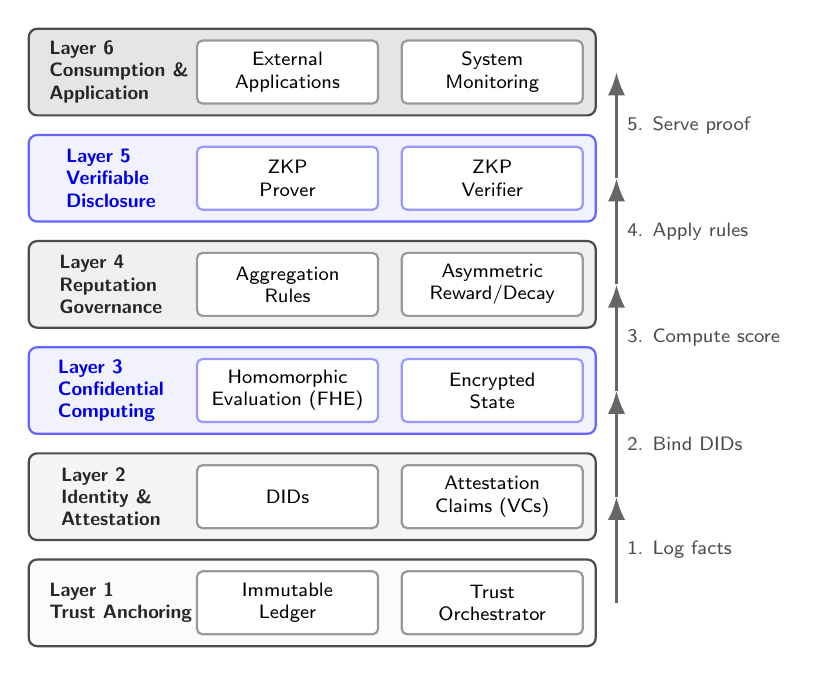
\begin{tikzpicture}[
    node distance=0.22cm,
    font=\sffamily,
    layer_box/.style={rectangle, draw=black!70, rounded corners=3px, minimum width=7.2cm, minimum height=1.1cm, thick, align=left},
    label_style/.style={font=\sffamily\bfseries\scriptsize, text=black!85, align=left, minimum width=1.8cm},
    comp_box/.style={rectangle, draw=black!40, fill=white, rounded corners=2px, font=\sffamily\scriptsize, minimum height=0.8cm, align=center, thick},
    flow_arrow/.style={-Latex, draw=black!60, line width=1.2pt},
    flow_lbl/.style={midway, right, font=\sffamily\scriptsize, text=black!70}
]
\node (L1) [layer_box, fill=gray!3] {};
\node [anchor=west, label_style, xshift=0.15cm] at (L1.west) {Layer 1\\Trust Anchoring};
\node [comp_box, minimum width=2.3cm] at ($(L1.west)+(3.3cm,0)$) {Immutable\\Ledger};
\node [comp_box, minimum width=2.3cm] at ($(L1.west)+(5.9cm,0)$) {Trust\\Orchestrator};
\node (L2) [layer_box, fill=gray!8, above=of L1] {};
\node [anchor=west, label_style, xshift=0.15cm] at (L2.west) {Layer 2\\Identity \&\\Attestation};
\node [comp_box, minimum width=2.3cm] at ($(L2.west)+(3.3cm,0)$) {DIDs};
\node [comp_box, minimum width=2.3cm] at ($(L2.west)+(5.9cm,0)$) {Attestation\\Claims (VCs)};
\node (L3) [layer_box, fill=blue!5, draw=blue!60, above=of L2] {};
\node [anchor=west, label_style, text=blue!90!black, xshift=0.15cm] at (L3.west) {Layer 3\\Confidential\\Computing};
\node [comp_box, draw=blue!40, minimum width=2.3cm] at ($(L3.west)+(3.3cm,0)$) {Homomorphic\\Evaluation (FHE)};
\node [comp_box, draw=blue!40, minimum width=2.3cm] at ($(L3.west)+(5.9cm,0)$) {Encrypted\\State};
\node (L4) [layer_box, fill=gray!12, above=of L3] {};
\node [anchor=west, label_style, xshift=0.15cm] at (L4.west) {Layer 4\\Reputation\\Governance};
\node [comp_box, minimum width=2.3cm] at ($(L4.west)+(3.3cm,0)$) {Aggregation\\Rules};
\node [comp_box, minimum width=2.3cm] at ($(L4.west)+(5.9cm,0)$) {Asymmetric\\Reward/Decay};
\node (L5) [layer_box, fill=blue!5, draw=blue!60, above=of L4] {};
\node [anchor=west, label_style, text=blue!90!black, xshift=0.15cm] at (L5.west) {Layer 5\\Verifiable\\Disclosure};
\node [comp_box, draw=blue!40, minimum width=2.3cm] at ($(L5.west)+(3.3cm,0)$) {ZKP\\Prover};
\node [comp_box, draw=blue!40, minimum width=2.3cm] at ($(L5.west)+(5.9cm,0)$) {ZKP\\Verifier};
\node (L6) [layer_box, fill=gray!20, above=of L5] {};
\node [anchor=west, label_style, xshift=0.15cm] at (L6.west) {Layer 6\\Consumption \&\\Application};
\node [comp_box, minimum width=2.3cm] at ($(L6.west)+(3.3cm,0)$) {External\\Applications};
\node [comp_box, minimum width=2.3cm] at ($(L6.west)+(5.9cm,0)$) {System\\Monitoring};
\draw [flow_arrow] ($(L1.east)+(0.25cm,0)$) -- ($(L2.east)+(0.25cm,0)$) node[flow_lbl] {1. Log facts};
\draw [flow_arrow] ($(L2.east)+(0.25cm,0)$) -- ($(L3.east)+(0.25cm,0)$) node[flow_lbl] {2. Bind DIDs};
\draw [flow_arrow] ($(L3.east)+(0.25cm,0)$) -- ($(L4.east)+(0.25cm,0)$) node[flow_lbl] {3. Compute score};
\draw [flow_arrow] ($(L4.east)+(0.25cm,0)$) -- ($(L5.east)+(0.25cm,0)$) node[flow_lbl] {4. Apply rules};
\draw [flow_arrow] ($(L5.east)+(0.25cm,0)$) -- ($(L6.east)+(0.25cm,0)$) node[flow_lbl] {5. Serve proof};
\end{tikzpicture}%
}
\caption{Layered architecture for privacy-preserving decentralized reputation.}
\label{fig:layered_architecture}
\end{figure}

\subsection{Framework Instances}
Different models are instantiated by changing mainly the Confidential Computing and Governance layers. In \textbf{Instance A (Verifiable Anonymous Reputation)}, confidential computing runs on the agent side via FHE, so the agent holds the keys and knows its own score, and governance operates in an open network that randomly assigns proposer and challenged roles. In \textbf{Instance B (Blind Reputation)}, confidential computing uses Secure Multi-Party Computation (MPC) combined with FHE distributed among a group, so that not even the subject knows its exact score, and governance moves to a permissioned environment with collective management. Instance A thus favors individual sovereignty, whereas Instance B trades individual knowledge for robustness against agents that tailor their behavior to a known score.

\section{ShadowRep: A Proof of Concept}\label{sec:poc}
ShadowRep realizes Instance A.\footnote{Source code: \url{https://github.com/mateus-n00b/bbyor}} Trust anchoring is provided by a Solidity contract that acts as oracle and hosts the Groth16 verifier, identity and attestation by W3C DIDs registered on a Hyperledger Indy ledger and managed by ACA-Py agents, which authenticate each other through DID Exchange over DIDComm \cite{hardman2019aries}, confidential computing by OpenFHE-Python \cite{openfhe2022} with the BFV scheme, governance by a reputation daemon integrated with the contract, and verifiable disclosure by a Groth16 circuit built with Circom and SnarkJS. Each peer is bound to a DID and to an account, and peers are admitted by the contract owner. This permissioned admission suits the evaluation, whereas an open deployment of Instance A would replace it with stake- or attestation-based admission. The target scenario is an Industrial IoT Cyber-Physical System (CPS) \cite{chang2013trust} in an Edge Computing environment, in which devices collaborate on tasks ranging from autonomous decisions to computational offloading. For instance, two thermostats collect temperature readings from a boiler, while a monitoring application tracks the reputation of each device and lowers it whenever the device misbehaves. Devices use the blockchain but do not take part in consensus. Fig.~\ref{fig:fluxo} shows the interaction between nodes and the contract in each round.

\begin{figure}[t]
\centering
\resizebox{\columnwidth}{!}{%
\begin{sequencediagram}
\newthread{prop}{Proposer}
\newinst[2]{chal}{Challenged node}
\newinst[2]{contract}{Smart contract}
\begin{sdblock}{Loop}{each round}
  \begin{call}{contract}{advance(): close round $t{-}1$, select proposer, draw $b$}{contract}{}
  \end{call}
  \begin{call}{prop}{Encrypt $\mathit{ct}_a$, compute $c''$ and $h$}{prop}{}
  \end{call}
  \begin{call}{prop}{commit$(t, h)$}{contract}{}
  \end{call}
  \begin{sdblock}{Opt}{not yet connected}
    \begin{call}{chal}{Connect (DIDComm), request challenge}{prop}{}
    \end{call}
  \end{sdblock}
  \begin{call}{prop}{Challenge $(t, \mathit{ct}_a)$}{chal}{}
  \end{call}
  \begin{call}{chal}{Read round $t$}{contract}{$b$, $h$, proposer}
  \end{call}
  \begin{call}{chal}{EvalAdd, Groth16 proof $\pi$}{chal}{}
  \end{call}
  \begin{call}{chal}{submitProof$(t, \pi)$}{contract}{$\alpha \gets \alpha + 1$}
  \end{call}
\end{sdblock}
\end{sequencediagram}%
}
\caption{PoE-FHE interaction in each round. Any account may call \texttt{advance()}, which applies Eq.~\eqref{eq:global} to the previous proposer once its window has closed.}
\label{fig:fluxo}
\end{figure}

\subsection{The PoE-FHE Challenge}\label{sec:poe}
In each round $t$, the contract selects a proposer (never the same twice in a row), draws a nonce $b$ in the scalar field of BN254, fixes the number $\beta$ of eligible verifiers, and opens a window of 30 to 40~s. The proposer encrypts a random value as $\mathit{ct}_a$ and derives the expected result
\begin{equation}\label{eq:result}
  c'' = \mathrm{SHA256}\big(\mathrm{ser}(\mathrm{EvalAdd}(\mathit{ct}_a, b)) \,\|\, b\big)_{[0,31)},
\end{equation}
where the first 31 bytes of the digest form a field element and the plaintext added by EvalAdd is $b \bmod 65537$, the BFV plaintext modulus, while the full $b$ enters the hash. The proposer then computes $h = H(c'', b)$, where $H$ is the Poseidon hash \cite{grassi2021poseidon}, records $h$ in the contract, and only then sends $\mathit{ct}_a$ to its peers over DIDComm. Both $b$ and $h$ are therefore public and immutable before any peer answers.

Each challenged node accepts $\mathit{ct}_a$ only over a connection authenticated by the public DID of the round's proposer, reads $b$ and $h$ from the contract, computes $c''$ by Eq.~\eqref{eq:result}, and proves knowledge of $c''$ such that
\begin{equation}\label{eq:poe}
  H(c'', b) = h,
\end{equation}
keeping $c''$ as a private witness. The circuit takes $b$, $h$, and the submitter's account as public inputs, and the contract builds these inputs from its own storage and from the transaction sender. A proof is thus valid only for its round and for the account that submits it, and the contract accepts at most one confirmation per verifier, so $\alpha \leq \beta$.

Equation~\eqref{eq:poe} holds for honest parties because the computation is deterministic. In BFV, adding a plaintext to a ciphertext introduces no randomness, which is confined to the single encryption of $\mathit{ct}_a$. Determinism, however, requires all parties to hash the same byte string. In OpenFHE, a freshly encrypted ciphertext serializes differently from one that has been deserialized, so the proposer derives $c''$ from the serialized $\mathit{ct}_a$ it sends, exactly as the challenged nodes do. Parties must also share the same parameters and library version, and hashing a canonical representation of the ciphertext polynomials would remove this dependency.

A malicious proposer may commit an invalid $h$. No honest node can then satisfy~\eqref{eq:poe}, the proposer receives no confirmations, and the severe penalty $\rho_0$ (Section~\ref{sec:model}) falls on the proposer itself. The attack is thus self-defeating. A proposer that never commits is penalized the same way. However, a round without confirmations looks the same whether the proposer misbehaved or its neighbors withheld their responses, so colluding neighbors could still lower an honest proposer's score. Committing a digest of $\mathit{ct}_a$ as well would enable a dispute phase in which anyone recomputes $c''$, and revealing $\mathit{ct}_a$ is harmless because it cannot be decrypted without the proposer's key.

\subsection{Reputation Model}\label{sec:model}
The contract manages a global reputation $\Gamma \in [0,1]$ of each agent as proposer. Every new identity starts at $\Gamma_0 = 0.35$, and when a round closes the proposer's score is updated as
\begin{equation}\label{eq:global}
  \Gamma_{t+1} = \begin{cases}
    \Gamma_t \cdot \rho_0, & \text{if } \alpha = 0, \\
    \Gamma_t \cdot \rho_1, & \text{if } 0 < \alpha < \tfrac{2}{3}\beta, \\
    \min\!\left(1,\; \Gamma_t + \tfrac{\alpha}{\beta}\,\delta\right), & \text{if } \alpha \geq \tfrac{2}{3}\beta,
  \end{cases}
\end{equation}
where $\alpha$ is the number of valid confirmations and $\beta$ the number of eligible verifiers, i.e., the admitted peers other than the proposer, fixed when the round opens. Rewards are additive ($\delta = 0.02$) and penalties multiplicative, reflecting that trust is hard to build and quick to lose. A partial failure applies $\rho_1 = 0.80$, while a round without valid confirmations, including one in which the proposer never commits $h$, applies $\rho_0 = 0.50$. These rules target the malicious behaviors identified for CPS \cite{chang2013trust}, namely \textit{dishonest behavior}, in which a node deliberately refuses the service or supplies incorrect information, \textit{incapacity or inconsistency}, in which it lacks resources or delivers degraded data, and \textit{systemic failures} that increase the risk for a group of agents.

\subsection{Threat Model}\label{sec:threats}
Nodes may be honest, faulty, or malicious. The critical assets are FHE private keys, ZKP witnesses, on-chain scores, and the integrity of PoE-FHE. We assume a computationally bounded adversary and an honest-but-curious blockchain. Table~\ref{tab:threat_model} summarizes the threats.

\begin{table}[t]
\centering
\caption{Threats, mitigations, and residual risk in ShadowRep.}
\label{tab:threat_model}
\footnotesize
\setlength{\tabcolsep}{2.5pt}
\renewcommand{\arraystretch}{1.05}
\begin{tabular}{@{}>{\raggedright}p{0.45cm}>{\raggedright}p{1.85cm}>{\raggedright}p{3.35cm}>{\raggedright\arraybackslash}p{2.35cm}@{}}
\toprule
\textbf{\#} & \textbf{Threat} & \textbf{Mitigation} & \textbf{Residual risk}\\
\midrule
T1a & Proof forgery & Groth16 verified on-chain, invalid proofs rejected & Negligible (see text)\\
T1b & Skipped execution & Proof bound to the on-chain commitment $h$ & Moderate, proves preimage knowledge only\\
T2 & Score inference & Challenge computed over FHE ciphertexts & High in PoC, $\Gamma$ stored in plaintext\\
T3 & Replay, duplicates & Public inputs $(b, h, \text{account})$ built on-chain, one confirmation per verifier & Low\\
T4 & Sybil, whitewashing & DIDs bound to accounts, admission by contract owner, newcomers start at $\Gamma_0$ & Low under admission control\\
T5 & Collusion & Random proposer selection, $\frac{2}{3}$ threshold & Moderate, large-scale collusion not addressed\\
T6 & FHE key theft & Keys held agent-side, DIDComm encryption & High if device is compromised (out of scope)\\
T7 & Oracle manipulation & Immutable contract, nonce and selection derived on-chain & Moderate in PoC, randomness biasable by block producer\\
T8 & Denial of service & One round at a time, window limits challenges & Low\\
T9 & Challenge poisoning & $h$ committed on-chain, invalid $h$ penalizes the proposer & Moderate, fault not attributable without dispute\\
T10 & Proposer impersonation & Challenges accepted only over connections authenticated by the proposer's public DID & Low\\
\bottomrule
\end{tabular}
\end{table}

For \textbf{T1a}, Groth16 is knowledge-sound in the generic and algebraic group models under the $q$-DLog assumption \cite{groth2016size, fuchsbauer2018algebraic}, so forging a proof without a valid witness is negligible, provided that discrete logarithms are hard on BN254 (about 100-bit security \cite{kim2016extended}), that the trusted setup is intact, and that Poseidon is preimage resistant. Our circuit-specific setup builds on a public multi-party Powers of Tau ceremony but uses a single contributor in its second phase, which suffices for evaluation, whereas deployment requires a multi-party second phase. Knowledge soundness does not, however, show that $c''$ was computed through EvalAdd (\textbf{T1b}). Since all neighbors receive the same $\mathit{ct}_a$ and $b$, a node may relay $c''$ to a colluding peer, which can then prove under its own account without having contacted the proposer. Binding proofs to accounts prevents the reuse of proofs, but not of witnesses. Admission control limits Sybil identities and whitewashing (\textbf{T4}), since re-registering requires the owner's approval; in an open deployment, lowering $\Gamma_0$ or delaying the use of newcomers' scores would discourage nodes whose score has decayed below $\Gamma_0$ from re-registering. In the PoC, $\Gamma$ is stored in plaintext in the contract (\textbf{T2}), and replacing it with commitments and threshold proofs is the role of the Verifiable Disclosure layer. The nonce and the proposer are derived from \texttt{prevrandao} and the previous block hash (\textbf{T7}), which a block producer can bias, so a deployment should use commit-reveal or a verifiable random function. Physical device compromise, ledger partitions, and key rotation are out of scope.

\section{Evaluation}\label{sec:eval}

\subsection{Experimental Setup}\label{sec:experiments}
All components ran as containers on a single host (Intel Core i7-1355U, 32~GB of RAM, Ubuntu 22.04), as depicted in Fig.~\ref{fig:exp_setup}. The network comprises 20 nodes, each pairing a ShadowRep daemon (Python 3.12) with its own ACA-Py 1.2 agent. DIDs are registered on a local Hyperledger Indy ledger (von-network), and the contract and its Groth16 verifier run on a local Hardhat network that produces a block every second. BFV uses plaintext modulus 65537 and multiplicative depth 2. All nodes are admitted to the contract at deployment and open DIDComm connections to every other node at start-up, so the topology is a full mesh from the first round and $\beta = 19$.

In each round, the contract selects one proposer at random (never twice in a row), draws the nonce $b$, and opens a 30 to 40~s window. The session lasted 460 rounds, or about 23 selections per node. Four nodes (20\%) were configured as anomalous through an environment variable read by the daemon, and the other 16 follow the protocol. Two nodes suffer \textbf{random omission failures}, skipping the proposal with probability 0.3 whenever selected (incapacity), and two are \textbf{on-off attackers}, which cooperate until $\Gamma \geq 0.6$ and then stop proposing (dishonest behavior). Anomalies act only in the proposer role, whose reputation is evaluated, so anomalous nodes still answer challenges normally. The baseline was measured in a second session of 416 rounds with the same topology.

\begin{figure}[t]
\centering
\resizebox{\columnwidth}{!}{%
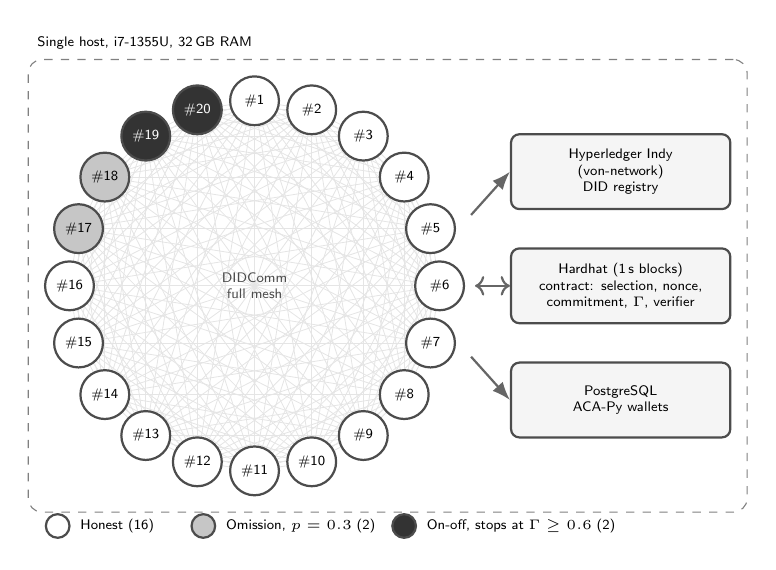
\begin{tikzpicture}[
    font=\sffamily\scriptsize,
    nd/.style={circle, draw=black!70, thick, minimum size=0.62cm, inner sep=0pt, font=\sffamily\tiny},
    honest/.style={nd, fill=white},
    faulty/.style={nd, fill=gray!45},
    attacker/.style={nd, fill=black!80, text=white},
    infra/.style={rectangle, rounded corners=3pt, draw=black!70, thick, fill=gray!8, align=center, text width=2.55cm, minimum height=0.95cm, font=\sffamily\tiny},
    lk/.style={-Latex, draw=black!60, thick}
]
\foreach \i in {1,...,20} {
  \foreach \j in {\i,...,20} {
    \ifnum\i<\j
      \draw[black!10, line width=0.3pt] ({90-(\i-1)*18}:2.35cm) -- ({90-(\j-1)*18}:2.35cm);
    \fi
  }
}
\foreach \i in {1,...,20} {
  \def\sty{honest}
  \ifnum\i=17 \def\sty{faulty}\fi
  \ifnum\i=18 \def\sty{faulty}\fi
  \ifnum\i=19 \def\sty{attacker}\fi
  \ifnum\i=20 \def\sty{attacker}\fi
  \node[\sty] (n\i) at ({90-(\i-1)*18}:2.35cm) {\#\i};
}
\node[align=center, font=\sffamily\tiny, text=black!70] at (0,0) {DIDComm\\full mesh};
\node[infra] (indy) at (4.65, 1.45) {Hyperledger Indy\\(von-network)\\DID registry};
\node[infra] (eth)  at (4.65, 0.0) {Hardhat (1\,s blocks)\\contract: selection, nonce,\\commitment, $\Gamma$, verifier};
\node[infra] (pg)   at (4.65,-1.45) {PostgreSQL\\ACA-Py wallets};
\draw[lk] (2.75, 0.9) -- (indy.west);
\draw[lk, <->] (2.8, 0.0) -- (eth.west);
\draw[lk] (2.75,-0.9) -- (pg.west);
\node[draw=black!50, dashed, rounded corners=5pt, fit=(n1)(n11)(n6)(n16)(indy)(pg), inner sep=0.2cm,
      label={[font=\sffamily\tiny, anchor=south west]north west:Single host, i7-1355U, 32\,GB RAM}] {};
\node[honest, minimum size=0.3cm] (lg1) at (-2.5,-3.05) {};
\node[anchor=west, font=\sffamily\tiny] at (lg1.east) {Honest (16)};
\node[faulty, minimum size=0.3cm] (lg2) at (-0.65,-3.05) {};
\node[anchor=west, font=\sffamily\tiny] at (lg2.east) {Omission, $p=0.3$ (2)};
\node[attacker, minimum size=0.3cm] (lg3) at (1.9,-3.05) {};
\node[anchor=west, font=\sffamily\tiny] at (lg3.east) {On-off, stops at $\Gamma\geq0.6$ (2)};
\end{tikzpicture}%
}
\caption{Experimental setup. Labels follow Fig.~\ref{fig:heatmap}.}
\label{fig:exp_setup}
\end{figure}

\begin{figure*}[t]
\centering
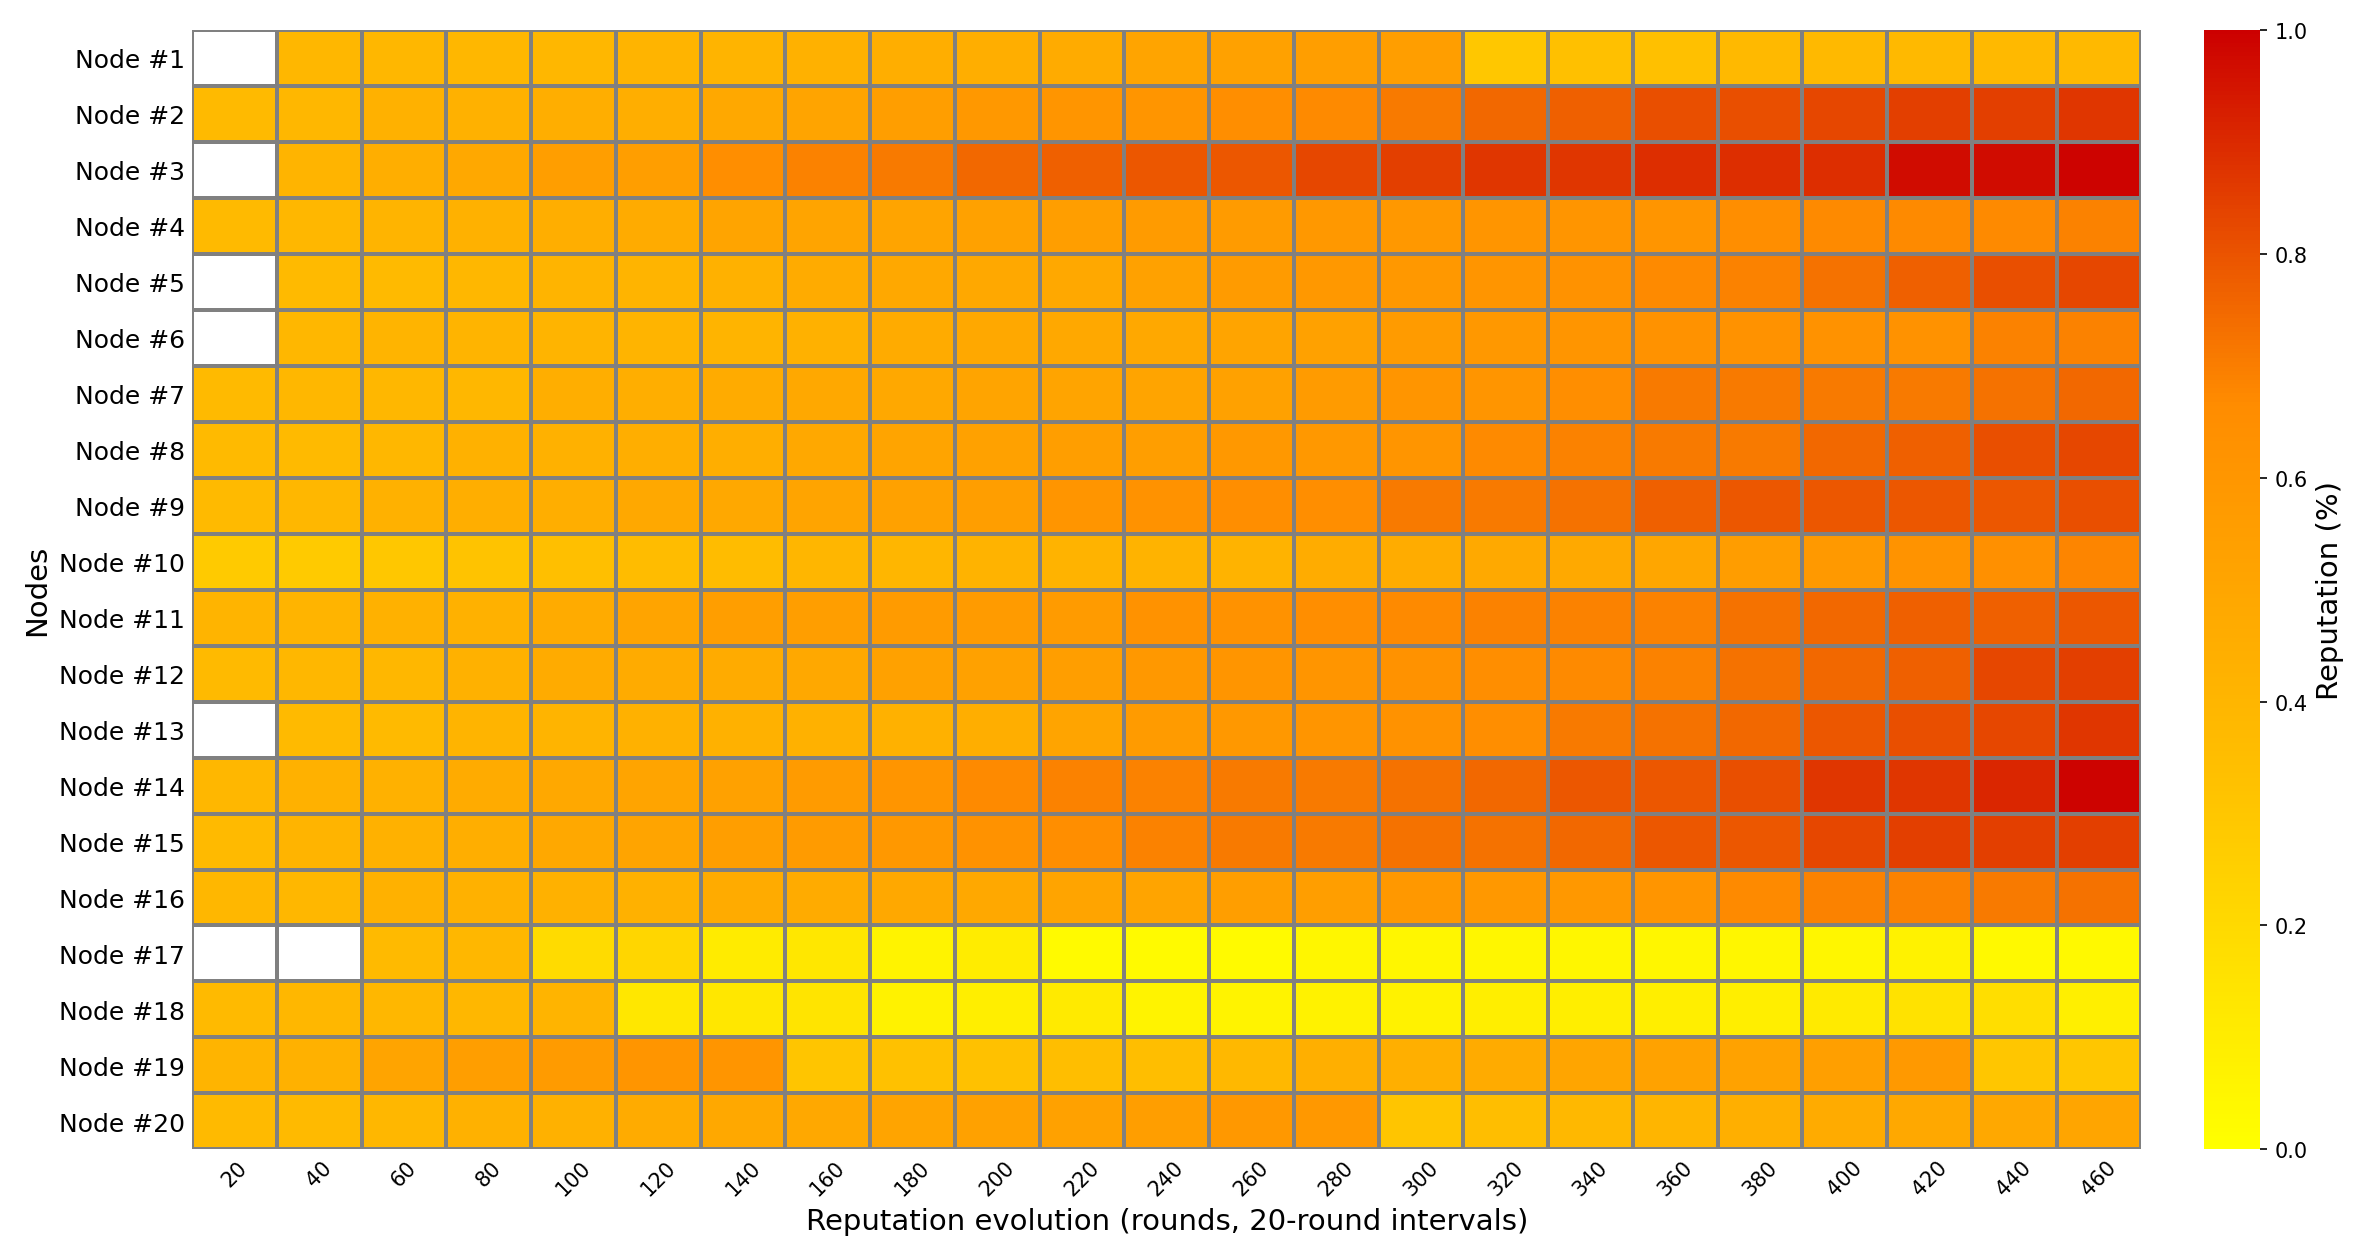
\includegraphics[width=0.85\textwidth]{images/reputation_rounds.png}
\caption{Global reputation per node in blocks of 20 rounds. Nodes \#1 to \#16 are honest, \#17 and \#18 have omission failures, and \#19 and \#20 are on-off attackers. Blank cells precede a node's first selection.}
\label{fig:heatmap}
\end{figure*}

The Hardhat network executes the contract and the on-chain Groth16 verification, but it runs as a single node without consensus. The results therefore omit block propagation and finality latency. We expect this effect to be limited, as BFT consensus in permissioned networks (e.g., QBFT) achieves block periods of a few seconds and reputation updates are asynchronous.

\subsection{Reputation Dynamics}
Fig.~\ref{fig:heatmap} shows the global reputation of each node in blocks of 20 rounds.

\textbf{Honest nodes (\#1 to \#16).} Honest proposers obtained a full quorum ($\alpha = \beta = 19$) in 367 of their 369 rounds (99.5\%), and their scores grow linearly with the number of times they were selected. The two nodes selected most often (32 times) reach 0.99, and the others end between 0.68 and 0.87 after 17 to 26 selections, so the spread among honest nodes reflects the randomness of proposer selection rather than differences in behavior. Two rounds deviate from this pattern. In round 7, node \#10 received only 2 confirmations, while peers were still completing their DIDComm connections, and was penalized by $\rho_1$. In round 303, node \#1 received none, owing to a transient failure whose cause could not be determined post hoc, and was halved from 0.55 to 0.275, ending the session at 0.375. Since a single failure offsets about 14 successful rounds, the rule favors fast detection over tolerance of isolated faults, and it cannot tell the root cause of a failure.

\textbf{Omission failures (\#17, \#18).} These nodes skipped 12 of their 37 proposals (32\%, in line with $p = 0.3$), fell below 10\% after rounds 162 and 163, and ended at 0.035 and 0.086. This level matches the equilibrium of Eq.~\eqref{eq:global}: with success probability $p_s = 0.7$, the expected gain $p_s\,\delta$ balances the expected loss $(1-p_s)(1-\rho_0)\,\Gamma$ at $\Gamma^{*} = p_s\delta / \big((1-p_s)(1-\rho_0)\big) \approx 0.09$.

\textbf{On-off attackers (\#19, \#20).} Both follow a sawtooth pattern. Each needed 13 successful proposals to climb from $\Gamma_0 = 0.35$ to 0.61, at which point it stopped proposing and was halved to 0.30, below its initial score. Returning to the threshold required 15 more successful proposals, so node \#19 defected only twice in 460 rounds (rounds 143 and 440) and node \#20 only once (round 293), ending at 0.30 and 0.51. Each defection thus costs the attacker about 15 honest services, and its reputation is never sustained at the level at which the attack would pay off.

Compared with our earlier prototype, the honest dynamics now reflect the rule itself. Responses complete well within the window, so honest proposers are no longer penalized by late confirmations, and the contract accepts at most one confirmation per verifier, so $\alpha$ never exceeds $\beta$.

\subsection{Computational Performance}
Table~\ref{tab:performance} compares the operations performed by a challenged node in PoE-FHE with a baseline of SHA-256 hashing and ECDSA signatures over secp256k1 (EIP-191 signing with public-key recovery). The computation step deserializes $\mathit{ct}_a$, evaluates $\mathrm{EvalAdd}$, and projects the result into a field element, taking 19.4~ms against 0.03~ms for hashing a plaintext. Proof generation dominates the cost at 236~ms, about 65\% of the total. Verification is now measured where it actually occurs: submitting a proof to the contract, which verifies it on-chain, takes 104~ms and about 273k gas, whereas the baseline proposer verifies each signature locally in 9.7~ms. On a like-for-like scope, i.e., computing the result and producing its attestation, PoE-FHE takes 256~ms against 7.9~ms, or roughly 33$\times$.

On the proposer side, creating the challenge (encryption, serialization, and the expected result) takes 28.6~ms. Computing the Poseidon commitment $h$ natively takes 2.4~ms, and committing it on-chain takes 36.6~ms and about 50k gas. With the round transition (about 101k gas), a round with 19 verifiers costs about 5.3~Mgas, which grows linearly with the number of verifiers. Each challenge also carries a BFV ciphertext of about 385~KiB, sent to every connection.

Proof generation is about 22$\times$ faster than in our earlier prototype (5.2~s). Most of the earlier cost came from the command-line pipeline, which launched one process per step (witness, proof, local verification, and calldata export) for every proof and made the proposer generate a proof only to compute $h$. A persistent prover process and a native Poseidon computation remove this overhead and, with shorter proofs, the CPU contention among co-located nodes.

\begin{table}[t]
\centering
\caption{Mean latency (95\% CI) per operation over 8{,}400 FHE+ZKP and 7{,}578 baseline responses.}
\label{tab:performance}
\footnotesize
\setlength{\tabcolsep}{3pt}
\begin{tabular}{@{}lrr@{}}
\toprule
\textbf{Operation} & \textbf{FHE+ZKP} & \textbf{Baseline}\\
\midrule
\multicolumn{3}{@{}l}{\textit{Challenged node}}\\
Computation (EvalAdd / SHA-256) & $19.4 \pm 0.3$~ms & $0.03$~ms \\
Proof / signature & $236.5 \pm 2.8$~ms & $7.8 \pm 0.1$~ms \\
On-chain submission and verification & $104.2 \pm 0.8$~ms & -- \\
Total per response & $361.0 \pm 3.4$~ms & $18.6 \pm 0.2$~ms \\
\midrule
\multicolumn{3}{@{}l}{\textit{Proposer}}\\
Challenge creation & $28.6 \pm 0.9$~ms & $0.04$~ms \\
Commitment $h$ (Poseidon) & $2.4 \pm 0.3$~ms & -- \\
Commitment transaction & $36.6 \pm 1.1$~ms & -- \\
Signature verification (per response) & -- & $9.7 \pm 0.1$~ms \\
\midrule
\multicolumn{3}{@{}l}{\textit{On-chain cost (gas)}}\\
Round transition / commitment / proof & \multicolumn{2}{@{}l}{$\approx$101k / 50k / 273k} \\
\bottomrule
\end{tabular}
\end{table}

The FHE+ZKP total includes the on-chain submission, and the baseline total includes sending the signed result back over DIDComm. In both cases, every response completes far within the 30~s minimum window, and since the daemon updates reputation asynchronously, it does not block the real-time tasks of the CPS, such as temperature readings. This cost buys zero-knowledge verifiability: a node proves that it holds a result consistent with the committed challenge without revealing it, and the proof cannot be replayed in another round or by another account, which signatures alone cannot provide.

\section{Discussion}\label{sec:discussion}
\textbf{Use of the score.} Depending on the policy adopted, applications may ignore agents whose reputation falls below a threshold (e.g., 10\%, which excluded both nodes with omission failures), and a token-based incentive can complement the penalties by rewarding correct behavior. The calibration factors ($\Gamma_0$, $\delta$, $\rho_0$, $\rho_1$, and the $\frac{2}{3}$ threshold) set clear trade-offs. The equilibrium $\Gamma^{*}$ determines how intermittent a node may be before it is excluded, the ratio between $\rho_0$ and $\delta$ fixes how many honest services an on-off attacker must render per defection, and the same ratio sets how long an honest node takes to recover from an isolated fault such as the one observed for node \#1. The same mechanism applies beyond IIoT, for instance to marketplaces, where anonymous feedback avoids retaliation, to social networks, where users build reputation without exposing their identity, to device monitoring, where PoE-FHE checks device health while preserving data confidentiality, and to the orchestration of AI agents, where a continuously monitored score discourages misbehavior during service provisioning.

\textbf{Limitations.} The evaluation ran on a single host and on a single-node ledger, so it does not capture network latency, consensus, or the contention patterns of physically distributed devices. On-chain verification grows linearly with the number of verifiers (about 273k gas each), which calls for aggregation or sampling of verifiers in larger networks. Proofs are now bound to the round's nonce and commitment and to the submitter's account, which closes replay and duplicate confirmations (T3). The commitment $h$ is recorded on-chain, but without a dispute phase the contract still cannot attribute a failed round to the proposer or to withholding neighbors (T9), and a verifier can still relay $c''$ to a colluding peer (T1b). In the PoC, the global score $\Gamma$ is kept in plaintext in the contract, so the Verifiable Disclosure of predicates over the score remains to be implemented. Finally, only the anonymous instance was evaluated.

\section{Conclusion}\label{sec:conclusao-e-trab-fut}
We presented a framework for decentralized reputation that integrates DIDs, ZKPs, and FHE through separate concerns, with two instances, anonymous and blind reputation. The ShadowRep proof of concept penalized omission failures and on-off attacks through proportional and auditable penalties, at a cost compatible with asynchronous updates. Future work includes implementing Blind Reputation (MPC and FHE), replacing plaintext scores with commitments and threshold proofs, adding a dispute phase that commits a digest of $\mathit{ct}_a$ to attribute failed rounds, aggregating or sampling verifier proofs to reduce on-chain cost, evaluating ShadowRep on a network with real consensus (e.g., Hyperledger Besu with QBFT) and on resource-constrained devices, and integrating it with mobile wallets.

\section*{Acknowledgments}
The authors acknowledge the support of the National Council for Scientific and Technological Development (CNPq) under grants 402854/2022-5 and 316208/2021-3, the Research Support Foundation of the State of Bahia (FAPESB) under grant TIC0004/2015, and the Air Force Office of Scientific Research (award number FA9550-23-1-0631).

\bibliographystyle{IEEEtran}
\bibliography{references}

\end{document}
